% LTeX: language=it

\chapter{Architettura del compilatore}
\label{chap:architettura-del-compilatore}

\begin{figure}[H]
	\centering
	\scalebox{0.8}{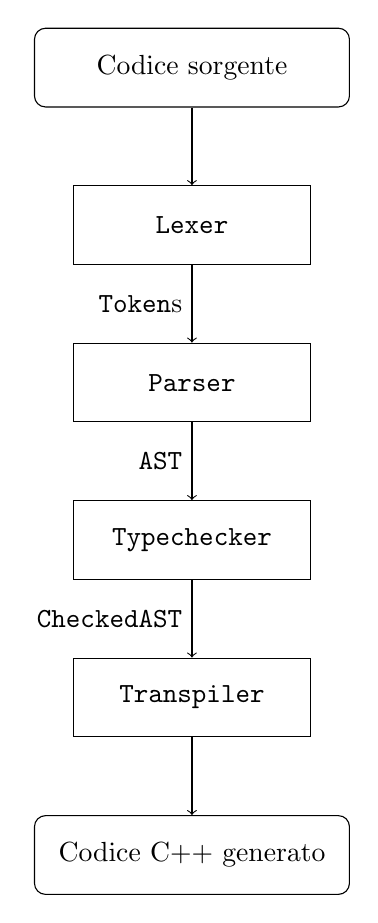
\begin{tikzpicture}[node distance=2cm]
		\node (source) [draw, rectangle, text centered, minimum width=4cm, minimum height=1cm, rounded corners] {Codice sorgente};
		\node (lexer) [below of=source, draw, rectangle, text centered, minimum width=3cm, minimum height=1cm] {\texttt{Lexer}};
		\node (parser) [below of=lexer, draw, rectangle, text centered, minimum width=3cm, minimum height=1cm] {\texttt{Parser}};
		\node (typechecker) [below of=parser, draw, rectangle, text centered, minimum width=3cm, minimum height=1cm] {\texttt{Typechecker}};
		\node (transpiler) [below of=typechecker, draw, rectangle, text centered, minimum width=3cm, minimum height=1cm] {\texttt{Transpiler}};
		\node (output) [below of=transpiler, draw, rectangle, text centered, minimum width=4cm, minimum height=1cm, rounded corners] {Codice C++ generato};

		\draw [->] (source) -- (lexer);
		\draw [->] (lexer) to node[left] {\texttt{Token}s} (parser);
		\draw [->] (parser) to node[left] {\texttt{AST}} (typechecker);
		\draw [->] (typechecker) to node[left] {\texttt{CheckedAST}} (transpiler);
		\draw [->] (transpiler) -- (output);
	\end{tikzpicture}}
	\caption{Moduli del processo di compilazione}
	\label{fig:moduli-compilatore}
\end{figure}

Nel seguente capitolo si descrive l'architettura del compilatore BugginOut, affrontando i moduli che lo compongono e le fasi del compilatore che realizzano. Nella figura sopra si pu\`o osservare l'architettura ad alto livello del compilatore che \`e costituito da quattro moduli principali:
\begin{itemize}
	\item \texttt{Lexer}: realizza l'analisi lessicale;
	\item \texttt{Parser}: realizza l'analisi sintattica;
	\item \texttt{Typechecker}: realizza l'analisi semantica;
	\item \texttt{Transpiler}: realizza la generazione del codice C++.
\end{itemize}
Questi interagiscono secondo un modello a \textit{pipeline}, in cui l'output di un modulo \`e l'input del successivo. Nel seguito si descriver\`a ciascuno di questi moduli e ci\`o che producono.

\section{\texttt{Lexer}}
\label{sec:lexer}

\begin{figure}[H]
	\centering
	\includegraphics[width=0.9\textwidth]{figures/lexer.png}
	\caption{Diagramma UML del \texttt{Lexer}}
	\label{fig:lexer-uml}
\end{figure}

L'analisi lessicale \`e realizzata per mezzo di due classi: \texttt{Token} e \texttt{Lexer}.

La classe \texttt{Token} rappresenta i token generati dall'analisi lessicale ed \`e costituito da:
\begin{itemize}
	\item \texttt{type}: il tipo del token (un valore dell'enumerazione \texttt{Token::Type});
	\item \texttt{value}: il valore del token (una stringa);
	\item \texttt{span}: la posizione del token nel codice sorgente (un oggetto di tipo \texttt{Span}\footnote{Questo tipo di oggetto rappresenta una posizione all'interno del codice sorgente ed \`e non altro che un intervallo di due indici nella stringa contenente il sorgente del programma.}).
\end{itemize}

La classe \texttt{Lexer} realizza l'automa a stati finiti discusso nella sezione \ref{sec:analisi-lessicale} memorizzando:
\begin{itemize}
	\item \texttt{source}: il codice sorgente da analizzare (una stringa);
	\item \texttt{current\_character}: il carattere da analizzare (un carattere);
	\item \texttt{current\_position}: la posizione del prossimo carattere da analizzare (un intero).
\end{itemize}
Il metodo \texttt{advance} permette di avanzare l'automa al prossimo carattere, aggiornando \texttt{current\_character} e \texttt{current\_position} e, inoltre, di controllare se si \`e raggiunti la fine del codice sorgente. In tal caso, il metodo imposta \texttt{current\_character} al valore speciale $-1$.

Con il metodo \texttt{next\_token} \`e possibile avanzare l'automa e generare il prossimo token. Ogni volta che questo metodo viene chiamato si occuper\`a di:
\begin{itemize}
	\item rimuovere spazi vuoti e commenti;
	\item analizzare \texttt{current\_character} e generare il token corrispondente o generare un errore se il carattere non \`e valido.\footnote{Per la gestione degli errori si veda la sezione \ref{sec:gestione-degli-errori}}
\end{itemize}
In base al carattere incontrato, si delega il compito dell'analisi lessicale ad uno dei metodi presenti nel diagramma. Ad esempio, se il carattere incontrato \`e un numero si richiamer\`a il metodo \texttt{lex\_number\_literal}. Questo permette di mantenere il codice del \texttt{Lexer} pulito e facilmente estendibile, poich\'e ogni metodo si occupa di un caso specifico.

\section{\texttt{Parser}}
\label{sec:parser}

\begin{figure}[H]
	\centering
	\includegraphics[width=0.9\textwidth]{figures/parser.png}
	\caption{Diagramma UML del \texttt{Parser}}
	\label{fig:parser-uml}
\end{figure}

L'analisi grammaticale \`e realizzata per mezzo della classe \texttt{Parser} e il gruppo di classi nel \textit{namespace} \texttt{AST}.

\section{\texttt{Typechecker}}
\label{sec:typechecker}

\section{\texttt{Transpiler}}
\label{sec:transpiler}

\section{Gestione degli errori}
\label{sec:gestione-degli-errori}
